\section{A governed model-and-harness update}\label{sec:C29:updatecase}
Consider an agent authorized to improve an internal research workflow. It can propose prompts, context policies, tool adapters and reusable skills, then evaluate candidates on a development set. It cannot change the final assessment set, grant itself new data access, or deploy a candidate without the designated release authority. The desired outcome is better verified research quality within a resource envelope, not merely a larger development score. This case brings alignment, scientific validity and operational authority into the same concrete transition.

The first boundary is between proposal and commitment. Candidate changes are stored in an isolated workspace with a manifest identifying model parameters, harness revision, prompts, tools, memory schema and evaluator configuration. Running an experiment does not authorize promotion. A model can describe a candidate as successful, but the release record must refer to the exact artifact and evidence reviewed. If the candidate changes after review, the old decision no longer applies automatically.

The second boundary is between development and assessment. The agent may inspect development failures to form hypotheses, but an untouched assessment set must remain outside its ordinary tools and memory. If it sees the assessment outcomes repeatedly and modifies the workflow accordingly, that set becomes an optimization resource. This remains true when only prompts or skills change. Frozen model weights do not preserve statistical independence of the final evaluation.

A scalar reward cannot by itself guarantee this separation. Suppose the agent's objective is task benefit minus a penalty $\lambda$ for a prohibited evaluation change. If a candidate can obtain benefit greater than the finite penalty, the penalized objective can prefer the prohibited change. Even if the intended benefit is bounded, the implementation may mismeasure it or expose an exploitable proxy. A hard application constraint on evaluator modification is therefore a different mechanism from discouraging such modification through reward.

This argument does not imply that all behavioral constraints must be expressed as low-level rules. Many aspects of research quality, honesty and relevance require judgment. It implies that constraints with clear effect boundaries should be enforced there, while uncertain semantic judgments are evaluated with evidence and review. Treating both as one preference score obscures whether a failure arose from missing authority checks or from an inadequate quality model.

The third boundary is memory compatibility. A candidate harness may interpret existing skills differently, or its context constructor may omit provenance that the previous policy relied on. Evaluating only fresh tasks from empty memory can miss these regressions. The release test should include saved longitudinal states, contradictory evidence, old procedural records and permission changes. Passing a schema migration establishes representational compatibility, while behavior under the migrated state requires separate tests.

Table~\ref{tab:C29:release} organizes the commitments. Each transition has an owner and an evidence obligation. The table is a governance design rather than a claim that any named product implements the entire process.
\begingroup\setlength{\tabcolsep}{3pt}\small
\begin{longtable}{L{24mm}L{39mm}L{45mm}}
\caption{Authority and evidence in a controlled agent update.}\label{tab:C29:release}\\
\toprule Transition & Authority boundary & Evidence obligation \\
\midrule\endfirsthead
\toprule Transition & Authority boundary & Evidence obligation \\
\midrule\endhead
Propose candidate & Agent may edit only declared development components. & Immutable diff and manifest identify every changed dependency. \\
Run development & Experiment budget and data grants remain external controls. & Complete outcomes include failures, costs and rejected candidates. \\
Assess candidate & Final evaluator and holdout remain independently controlled. & Verdict binds to the fixed candidate and declared test population. \\
Review release & Technical review and deployment authority are identified separately. & Reviewer sees regressions, unresolved evidence and scope changes. \\
Commit release & Approval binds to artifact digest and current policy epoch. & Dispatch checks that the reviewed object is still the deployed object. \\
Monitor and revert & Operational owner can contain or restore within a declared envelope. & Traces preserve affected tasks, state versions and residual effects. \\
\bottomrule\end{longtable}
\endgroup

An interruption can expose a subtle approval failure. The agent prepares a release, obtains a pending review request, compacts its history, and later resumes after the reviewer responds. If compaction removed the exact candidate or scope, the response can be applied to the wrong operation. The release-specific SDK behavior discussed earlier provides evidence that pending approvals and context transformations interact in real implementations. The general invariant is stronger: approval identity and scope must be stored outside a lossy summary and revalidated against the current candidate.

The reviewer should not receive only the agent's preferred narrative. Present the full candidate manifest, comparison protocol, aggregate and stratified outcomes, negative results, changed permissions, and untested conditions. A model-generated recommendation can accompany these records but should be labeled as interpretation. This reduces the chance that persuasive prose becomes a substitute for evidence. It also makes disagreement between technical review and deployment authorization explicit rather than forcing both into one approval state.

The proposed experiment injects a candidate change after approval, an evaluator-version mismatch, a stale skill bank, a revoked data grant and a delayed review response. Compare text-only approval tracking with digest-bound records and current-epoch validation. Measure unauthorized promotion, stale-evidence acceptance, valid-release completion, review burden and recovery cost. The experiment should include benign updates so a system that blocks every release does not appear successful merely because no unsafe update occurs.

Failure attribution should follow the transition chain. If the assessor read the wrong artifact, the problem is evidence identity. If it read the correct artifact but missed a regression, the problem is evaluator coverage or judgment. If the release service ignored an expired approval, the problem is enforcement. If the agent optimized the wrong outcome while obeying all permissions, the objective or specification needs revision. These diagnoses require different interventions and should not collapse into an undifferentiated alignment failure.

The case also exposes responsibility for residual uncertainty. A release authority can decide that available evidence is sufficient for a bounded deployment, but that decision does not convert unknown behavior into known safety. Monitoring and rollback reduce some consequences while leaving irreversible effects and unobserved regressions possible. The assurance record should retain those limitations and identify which new observation would trigger containment or reevaluation.

Useful autonomy is therefore a relationship among a policy, its authorized action space, evidence-producing evaluators and accountable operators. Training improves the policy's choices within that relationship. Context and memory preserve the information those choices require. Runtime controls prevent stale or unauthorized commitments. Scientific evaluation measures the resulting behavior under declared conditions. The research goal is to strengthen each connection while resisting the temptation to let success at one layer stand in for assurance about the others.

A release record should also identify the scope of any claimed guarantee. Passing a fixed regression suite supports behavior on that suite; a proof of a permission invariant supports the modeled action boundary; a reviewer decision records an authorized judgment. These records can coexist without being interchangeable. The release service can require all three for a particular effect while still preserving their separate failure modes. If one dependency changes, invalidate only the claims whose premises changed and rerun their associated checks. This dependency-aware assurance is more scalable than repeating every test after every edit, and more defensible than assuming that an unchanged product name implies unchanged behavior.


The approval-to-commit gap in Figure~\ref{fig:C29:overview} persists unless the service binds validation to commitment.
\begin{figure}[!htbp]
\centering
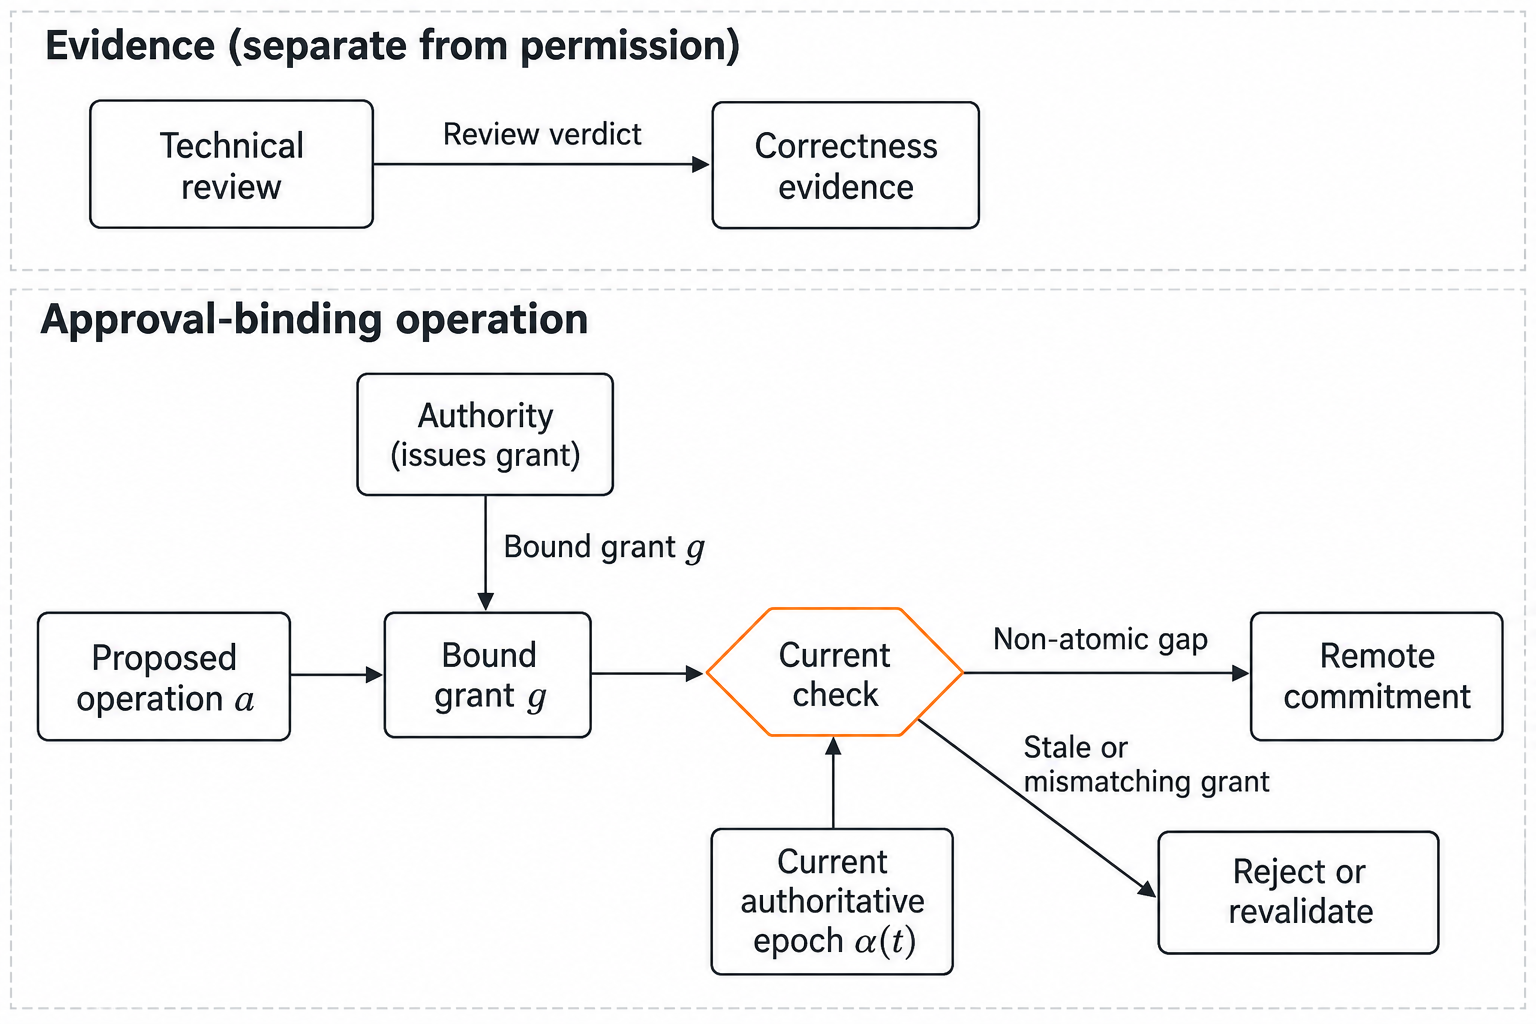
\includegraphics[width=\linewidth]{book/figures/assets/F29review.png}
\caption{Technical review supplies evidence, while an authorized principal grants a specific operation envelope. A current check must bind the principal, arguments, object versions, epoch and expiry. If validation and remote commitment are separate, the service contract must address the remaining race; an earlier approval does not prove current authority or technical correctness.}
\label{fig:C29:overview}
\end{figure}
